\section{Results}
\subsection{Vegetation classification}
The vegetation classification resulted in a map showing the different classes (figure \ref{fig:classification}). The data points which were removed during the preprocessing are displayed in grey. This class contains data points that certainly do not contain higher than herb vegetation, as it mainly contains bare soil, grassland and water bodies (compare figure \ref{fig:studyarea}). The blue class represents data points which were not removed during the preprocessing, but were classified as `other' during the supervised classification (mainly building edges, ditches and railroad infrastructure). The green class represents the classified vegetation. The accuracy of this classification is presented in a confusion matrix of predicted versus actual classes (table \ref{tab:confmatclass}). From the confusion matrix a producer’s accuracy of 0.98 for `vegetation' and of 0.85 for `other' was calculated. The AUROCC of 0.98 shows that `vegetation' and `other' class are separated well, which is supported by the MCC of 0.76, indicative of a positive correlation between the predicted and observed classes, and the geometric mean of 0.90.

\begin{figure}
	\centering
	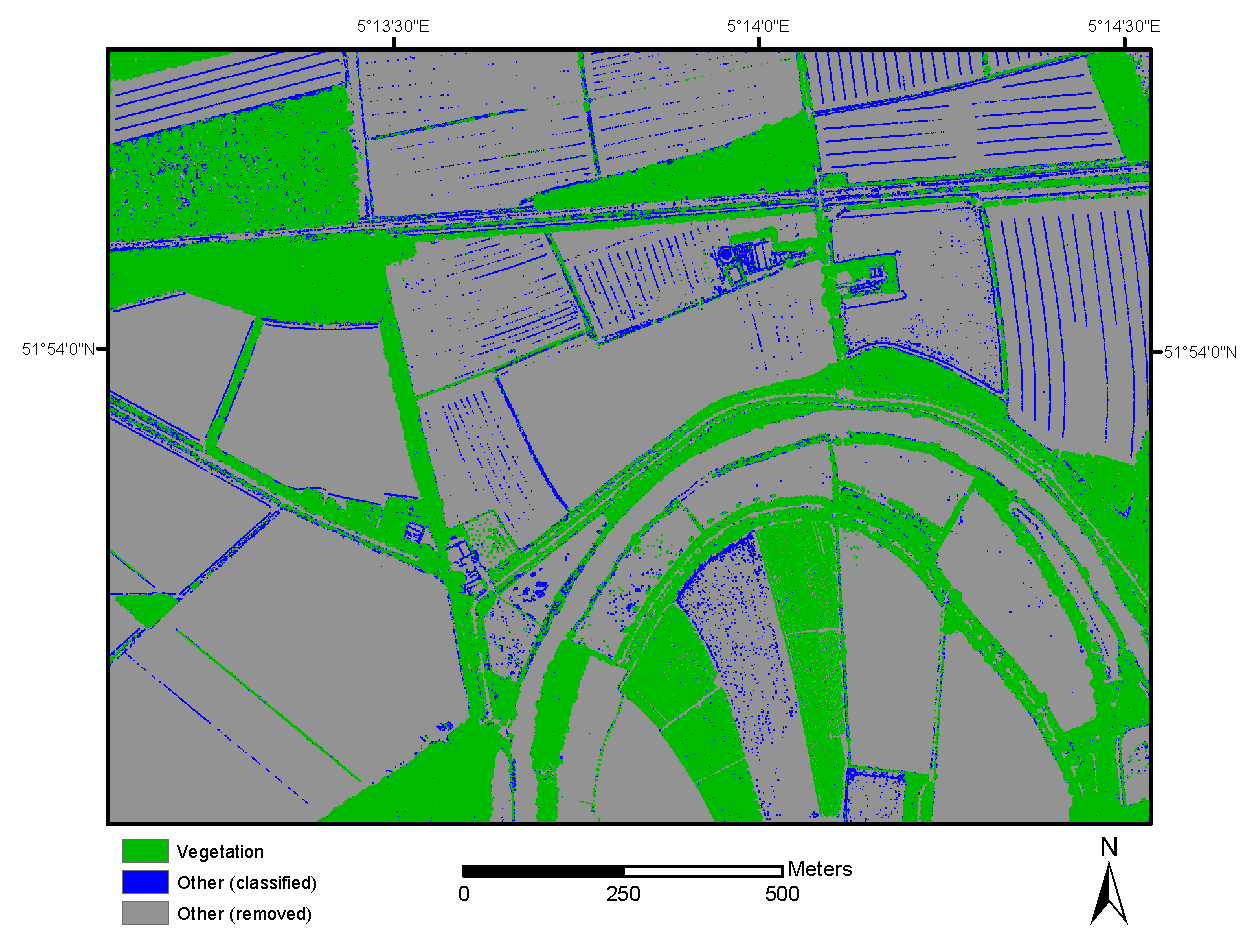
\includegraphics[width=\columnwidth]{./img/classification.pdf}
	\caption{Results of the vegetation classification. Grey areas represent data points which were removed during the preprocessing, blue represent data points which were not removed during the preprocessing, but classified as non-vegetation (mainly building edges, ditches and railroad infrastructure). Green represents the higher than herb vegetation.}
	\label{fig:classification}
\end{figure}

\begin{table}
	\caption{A confusion matrix showing the predicted classes against the actual classes of the points. These are accumulated over the 10 fold cross-validation.}
	\label{tab:confmatclass}
	\begin{tabular}{l l l l l l l}
		\toprule
		& & & \multicolumn{2}{c}{\textbf{Predicted}} & & \\
		& & & Vegetation & Other & & \\
		\midrule
		\parbox[t]{2mm}{\multirow{4}{*}{\rotatebox[origin=c]{90}{\textbf{Actual}}}} & & & & & & \\
		& Vegetation & & 974177 & 22908 & & \\
		& Other & & 8171 & 47999 & & \\
		& & & & & & \\
		\bottomrule
	\end{tabular}
\end{table}

\subsection{Linear object segmentation}
The vegetation was segmented using our region growing algorithm and the resulting objects were filtered for linearity. We compare the result with our manual segmentation (figure ..). The areas that were correctly classified as linear vegetation objects are shown in light green and the regions that were accurately classified as nonlinear vegetation objects are displayed in dark green. Nonlinear areas that are classified as linear are shown in red and linear regions that are classified as nonlinear are shown in orange.  A confusion matrix is used to quantify the accuracy of the automated segmentation (table \ref{tab:confmatseg}).

.. an overall accuracy of 0.87, F1 scores of 0.77, kappa of 0.70, and MCC of 0.70 respectively. Although there are some obvious errors, the majority of linear woody objects have been successfully segmented, with with user’s and producer’s accuracies of .. and .., respectively. Non-linear objects are successfully separated well, with user’s and producer’s accuracies of 0.90 and 0.93, respectively.

%\begin{table}
%	\caption{Confusion matrix listing the automatically segmented against the manually annotated set of linear and non-linear vegetation objects in area (\(m^{2}\)).}
%	\label{tab:confmatseg}
%	\begin{tabular}{l l l l l l l l}
%		\toprule
%		& & & \multicolumn{2}{c}{\textbf{Predicted}} & & & \\
%		& & & Linear & Nonlinear & & Producer's accuracy & \\
%		\midrule
%		\parbox[t]{2mm}{\multirow{4}{*}{\rotatebox[origin=c]{90}{\textbf{Actual}}}} & & & & & & & \\
%		& Linear & & 1159762 & 23438 & & & \\
%		& Nonlinear & & 6416 & 16706 & & & \\
%		& & & & & & & \\
%		& User's accuracy & & & & & & \\
%		\bottomrule
%	\end{tabular}
%\end{table}

\begin{table}
	\caption{Confusion matrix listing the automatically segmented against the manually annotated set of linear and non-linear vegetation objects in area (\(m^{2}\)).}
	\label{tab:confmatseg}
	\begin{tabular}{l l l l l l l}
		\toprule
		& & & \multicolumn{2}{c}{\textbf{Predicted}} & & \\
		& & & Linear & Nonlinear & & \\
		\midrule
		\parbox[t]{2mm}{\multirow{4}{*}{\rotatebox[origin=c]{90}{\textbf{Actual}}}} & & & & & & \\
		& Linear & & 1159762 & 23438 & & \\
		& Nonlinear & & 6416 & 16706 & & \\
		& & & & & & \\
		\bottomrule
	\end{tabular}
\end{table}